\capitulo{3}{Conceptos teóricos}

En este proyecto, la mayor completitud del trabajo se encuentra en el preprocesado de las imágenes, el cual es necesario uno distinto según la red con la que se trabaje.  

\section{Conceptos de Redes Neuronales Convolucionales}

    En este apartado se pondrá en contexto sobre los conceptos más importantes a tener en cuenta sobre una red neuronal convolucional, partiendo desde la idea de la inteligencia artificial.

    La inteligencia artificial es una tecnología que busca imitar la inteligencia humana, los objetivos de la inteligencia artificial son: representación de conocimientos, aprendizaje automático, procesamiento del lenguaje natural, inteligencia social e inteligencia general \cite{definicion_artificial_intelligence}.

    El aprendizaje automático, o \textit{machine learning}, es una rama de la inteligencia artificial, cuyo objetivo es que las máquinas aprendan por si mismas. Se considera aprendizaje la acción de mejorar el rendimiento en futuras acciones~\cite{machine-learning}. Dependiendo de la naturaleza, se puede considerar aprendizaje supervisado, aprendizaje no supervisado y aprendizaje por refuerzo.

    El aprendizaje automático como resultado da un modelo, que está basado en uno de los siguientes clasificadores:
    Árboles de decisión, reglas de asociación, algoritmos genéticos, máquinas de soporte vectorial, \textit{clustering}, redes bayesianas y redes neuronales artificiales.

    Las redes neuronales artificiales (RNN) son modelos computacionales con al menos una capa oculta\cite{definicion_neural_network}, la cual consiste en una o más neuronas donde cada una calcula la suma de los valores de entrada, multiplicados por su peso correspondiente\cite{definicion_hidden_layer}.

    El valor calculado se utiliza en una función de activación, que produce el valor de salida\cite{definicion_activation_function}. Entre las funciones de activación destacan las visibles en \ref{fig:funciones de activacion}.
    \begin{itemize}
        \item La función RELU (verde), la cual indica el máximo entre 0 y el valor calculado.
        \item La función lineal(rosa), la cual devuelve el mismo valor calculado.
        \item La función sigmoidea(cían), la cual devuelve un valor entre 0 y 1 según lo alejado que este del 0.
        \item La función escalón(morada), devuelve o 0 o 1 dependiendo del signo del valor calculado.
    \end{itemize}
    
    \begin{figure}[!ht]
         \centering
         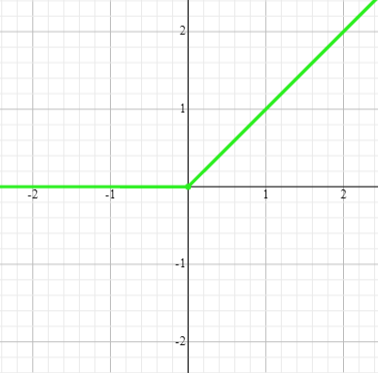
\includegraphics[width=0.45\textwidth]{img/RELU.png}
         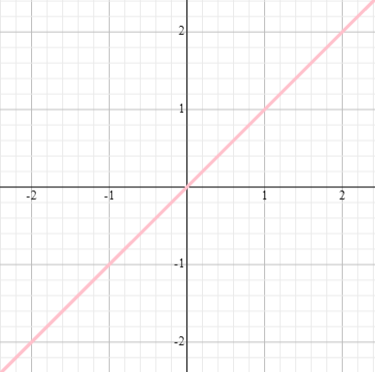
\includegraphics[width=0.45\textwidth]{img/lineal.png}

         \hfill \break
         \centering
         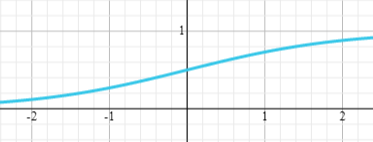
\includegraphics[width=0.45\textwidth]{img/Sigmoidal.png}
         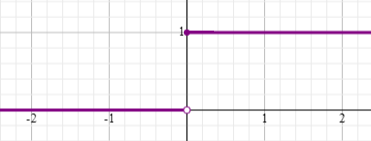
\includegraphics[width=0.45\textwidth]{img/escalon.png}
         
         \caption{Funciones de activación}
         \label{fig:funciones de activacion}
    \end{figure}

     Dentro de las redes neuronales, se encuentran las redes neuronales convolucionales (CNN), es una red neuronal en la que hay al menos una capa convolucional, consistiendo en la combinación de capas convolucionales, capas de agrupación y capas densas \cite{definicion_CNN}.

     Una capa convolucional es un conjunto de neuronas artificiales que realizan varias series de operaciones convolucionales, actuando cada una sobre una submatriz de la matriz de entrada \cite{definicionConvolucional_layer}.
     
     Una operación convolucional es aquella que a partir de una submatriz de la matriz de entrada, donde a veces es necesario realizar un filtrado, para ponderar los datos, calculando la suma de los valores de la submatriz, o en caso de que se haya realizado un filtro, del resultado de este, asignando el valor de la suma a una nueva matriz resultado con las dimensiones de la matriz de entrada \cite{definicionConvolutional_Operation}.
     
     La capa de agrupación es una capa de una red neuronal, es una capa que reduce el tamaño de la matriz de entrada, mediante operaciones como el máximo o la media de los valores de una submatriz\cite{definicion_pooling}.

     La capa densa también llamada capa totalmente conectada, es una capa oculta, donde cada nodo esta conectado a todos los nodos de la siguiente capa oculta\cite{definicion_fully_connected_layer}.
     
    Una red neuronal residual es una red que permite el salto de capas intermedias. Para ello, se crea un bloque residual, lo que hace es al resultado de la ruta residual, sumar la entrada del bloque a la salida del bloque, como se puede ver en \ref{fig:residual-block}

\begin{figure}[!ht]
         \centering
         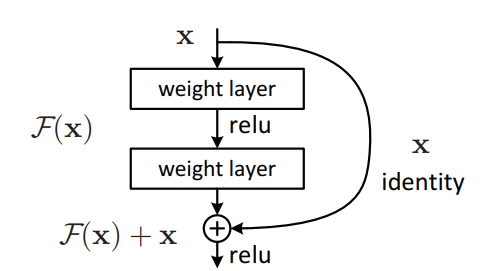
\includegraphics[width=0.6\textwidth]{img/residual-block.png}
         \caption{Bloque residual. Imagen extraída de \cite{DBLP:journals/corr/HeZRS15}}
         \label{fig:residual-block}
\end{figure}
\section{Preprocesado}
En el proyecto, se han realizado varios preprocesados, puesto que hay varias redes neuronales convolucionales.

\subsection{Red neuronal convolucional VGG16, para la calidad de la imagen}

En una red neuronal convolucional VGG16, el preprocesado necesario es que la imagen en vez de estar en formato RGB (Rojo verde y azul), tiene que ser formato BGR con los valores centralizados en 0. Además de este cambio, la imagen tiene que tener de 224 x 224 píxeles.
\cite{tensorflowVGG16}
Para realizar este preprocesado en Python, se puede llamar a la función \textit{tf.keras.applications.vgg16.preprocess\_input}, para la aplicación de Android Studio, se debe realizar este preprocesamiento a mano.
La estructura de la red convolucional VGG16, se puede observar en la figura \ref{fig:VGG-16-struct}, donde hay 13 capas convolucionales, y  4 de agrupación. 
\begin{figure}[!ht]
         \centering
         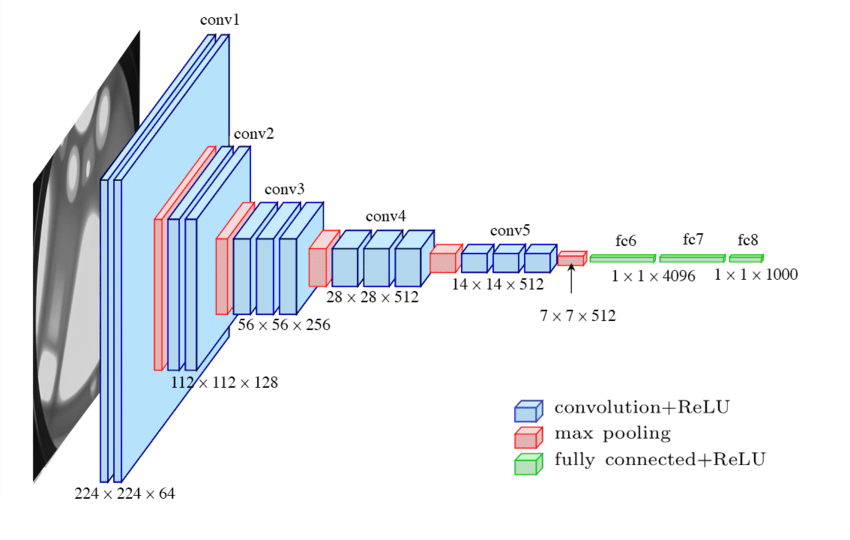
\includegraphics[width=0.9\textwidth]{img/VGG-16-network-architecture.png}
         \caption{Estructura básica de la red convolucional VGG16. Imagen extraída de \cite{vgg16-structure}}
         \label{fig:VGG-16-struct}
\end{figure}


\subsection{Red neuronal convolucional ResNet50V2, para la detección de retinopatía}

La red ResNet50V2 es una red neuronal residual que, como se ha comentado anteriormente, permite saltarse capas, como se puede ver en la figura \ref{fig:residual-block}.

En la red neuronal convolucional ResNet50V2, el procesamiento es distinto al de VGG16, la gama de color es RGB, también se tiene que normalizar los datos, pero en este caso, el intervalo es [-1,1]. \cite{tensorflowResNet50V2}

Esta red neuronal ya estaba entrenada, por tanto, no se tuvo que hacer ningún preprocesado en Python; pero al implementar la red en Android Studio, al igual que en la red VGG16, se debía realizar el preprocesamiento a mano.

Donde la formula para cambiar este valor vendría dada por: 
\begin{center}
    $ColorPreprocesado = (ColorSinPreprocesar - 0)/ 255.0 * 2 - 1$
    \begin{itemize}
        \item Donde 0 representa el valor mínimo que puede tomar el color en concreto.
        \item Donde 255 representa el valor máximo que puede tomar el color en concreto.
        \item Y donde $ * 2 - 1 $ es la operación para normalizar el valor en formato [-1, 1]
    \end{itemize}
\end{center}

La estructura de la red convolucional ResNet50V2, se puede observar en la figura \ref{fig:ResNet50v2-struct}, en esta red neuronal convolucional,  
\begin{figure}[!ht]
         \centering
         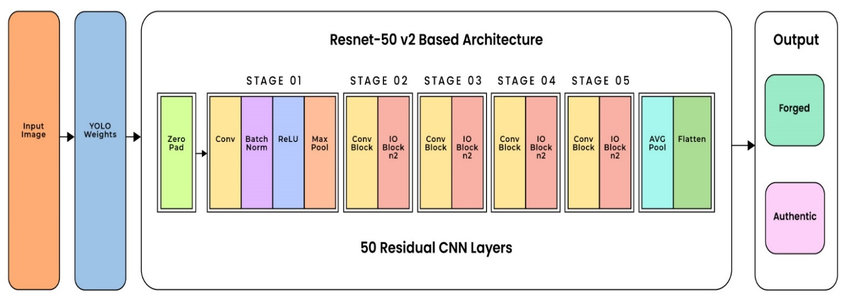
\includegraphics[width=0.9\textwidth]{img/ResNet50v2-architecture.jpg}
         \caption{Estructura básica de la red convolucional ResNet50v2. Imagen extraída de \cite{ResNet50v2-architecture}}
         \label{fig:ResNet50v2-struct}
\end{figure}

\section{Formato de la red neuronal}

El formato de las redes neuronales convolucionales suele venir dado en formato ``.h5'' o keras, para facilitar la implementación en Android Studio, se ha tenido que transformar este archivo en formato TensorFlow Lite, el cual requiere menos recursos, permitiendo su integración en dispositivos móviles.

Para realizar esta conversión, se ha utilizado un fichero Python, el cual se ha buscado en la documentación de TensorFlow Lite, y posteriormente, guardar el fichero. \cite{tensorflowliteConverter}

En el siguiente código, se puede observar el convertidor, donde file es el directorio donde se encontraría el archivo keras, nombre es el nombre de este fichero, y fileSalida es el directorio de salida.
\lstset{
  language=Python,
  basicstyle=\ttfamily,
  keywordstyle=\color{blue},
  commentstyle=\color{green!60!black},
  stringstyle=\color{red},
  showstringspaces=false,
  breaklines=true,
  breakatwhitespace=true,
  tabsize=4,
  numbers=none,
  numberstyle=\tiny,
  frame=single,
  framexleftmargin=5mm,
  xleftmargin=5mm
}
\begin{lstlisting}
model = tf.keras.models.load_model(file+nombre+'.h5')
converter = tf.lite.TFLiteConverter.from_keras_model(model)
tflite_model= converter.convert()
nombreSalida = "calidad.tflite"
with open(fileSalida+nombre+'.tflite', 'wb') as f:
    f.write(tflite_model)

\end{lstlisting}
\section{Desbalanceo de los datos}

Para la minería de datos, el problema de que los datos estén desbalanceados causa que los modelos entrenados suelan producir resultados indebidos.

Un ejemplo del desbalanceo de datos, podría ser un modelo que entrena los números diciendo si son primos o no. En este caso, si se calcula el modelo por porcentaje de aciertos, en caso de devolver siempre que el número introducido no es primo, esta medida tiende a ser del 100\%.
Por este motivo, se suelen usar otras métricas u otras formas de entrenar al modelo, para que se evite la disparidad de los datos.

La forma de solucionar este problema en este trabajo ha sido usando otras medidas como podrían ser precisión, recall y F1Score.
En la figura \ref{fig:matrizDeConfusion} se puede observar la matriz de confusión de positivos y negativos. A partir de la cual, se explicaran las medidas.
\begin{figure}[!ht]
         \centering
         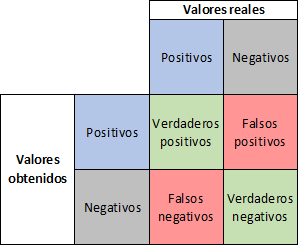
\includegraphics[width=0.6\textwidth]{img/Matriz de confusion.png}
          \caption{Matriz de confusión}
         \label{fig:matrizDeConfusion}
\end{figure}

La precisión es el numero de Verdaderos positivos entre la suma de verdaderos positivos y falsos positivos.
\begin{center}
    $Precision = \dfrac{Verdaderos Positivos} {Verdaderos Positivos + Falsos Positivos} $
\end{center}

Por otro lado, el recall, es el número de verdaderos positivos entre la suma de los verdaderos positivos y los falsos negativos.
\begin{center}
    $Recall = \dfrac{Verdaderos Positivos} {Verdaderos Positivos + Falsos Negativos} $
\end{center}

F1 Score es una medida obtenida de las dos anteriores, siendo la media armónica de estas.
\begin{center}
    $F_1 = 2 \dfrac{Precision * Recall} {Precision + Recall} $
\end{center}

En el caso concreto, una imagen puede ser APTA o NO\_APTA, encontrándose el desbalanceo de imágenes de 455 APTA y 103 NO\_APTA. De esta forma, se ha considerado en la matriz \ref{fig:matrizDeConfusion}, como ``Positivos'' a la clase NO\_APTA y como ``Negativos'' a la clase APTA.

La otra opción que no se ha utilizado, pero es importante destacarla, es el uso de oversampling o undersampling. Estas técnicas buscan igualar número de entidades en el conjunto de datos según la clase. 

Mientras oversampling, busca añadir datos a partir del conjunto de datos, duplicando o modificando los datos entre distintas instancias. Esta opción no se ha ni planteado, puesto que si se duplican las imágenes NO\_APTA, lo que va a producir es sobreajuste del modelo; y suponiendo que los datos nuevos fuesen modificaciones de combinaciones de imágenes  NO\_APTA, se estaría introduciendo ruido, puesto que crearía imágenes no reales.

El undersampling al contrario que el oversampling, elimina datos del grupo mayoritario, hasta que hay un número similar de instancias, las instancias eliminadas se pueden utilizar para validación o para test. Al implementar este método, se pueden eliminar inicialmente instancias que clasifican muy bien el modelo, haciendo que dependa el código de la inicialización del conjunto de entrenamiento y del conjunto de test.